%% It is just an empty TeX file.
%% Write your code here.
\chapter{Dependability} \label{ch:dependability}

%************************************************************************************************************************%
\section{Taxonomy} \label{sec:tax}

What makes a system dependable and what does dependability actually mean? \\

\begin{figure}[H]
\centering
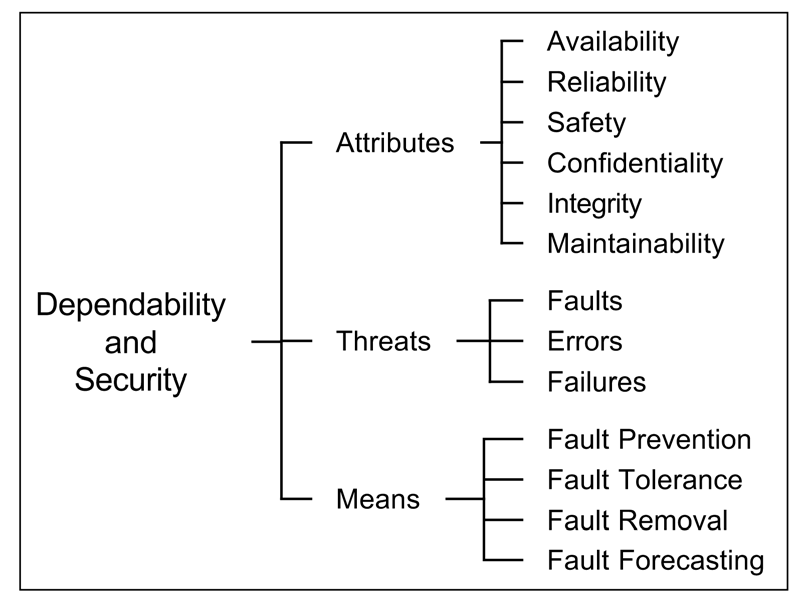
\includegraphics[width=0.65\textwidth]{figures/DepTax.PNG}
\caption{Dependability Taxonomy~\cite{art:Avizienis}}
\label{fig:deptax}
\end{figure}

The dependable system is a system, which has the ability to deliver it's service with acceptable number and severity of system failures~\cite{art:Avizienis}. Dependability ensures therefore the quality of the system's service~\cite{art:Laprie}. Above all the dependability is an integrating term that encapsulates following \textbf{attributes}:
\begin{itemize}
\item \textbf{availability} - readiness for the delivery of correct service, can be used as a  measure, being a time function $A(t)$ showing the probability that the system functions correctly at the particular time $t$. 
\item \textbf{reliability} - permanence in the delivery of correct service, can also be used as a measure, being the time function $R(t)$ showing the probability that the system has functioned correctly in the time interval $[t_0,t]$ under assumption that it has functioned correctly at the time $t_0$.
\item \textbf{safety} - absence of catastrophic system failures and ability to transit and reside in the fail-safe state, again a measure being a time function $S(t)$ showing probability that a system that worked correctly at time $t_0$ works correctly in the interval $[t_0,t]$ or remains in the fail-safe state,
\item \textbf{maintainability} - possibility of the system alteration and repairs (by authorized subjects) given as a time function $M(t)$ showing the probability that a faulty system will be repaired within time $t$~\cite{art:Laprie, art:Avizienis, art:Avizienis2}.
\end{itemize}
The mentioned above definitions are based on two important terms: system failure and correct service, being in fact antonyms. The absence of one means the presence of the other. A system failure is therefore one of the impairments that threaten the dependability. There are three \textbf{threats}, that form a hierarchical structure:
\begin{itemize}
    \item \textbf{failure} - a state when system delivers service that deviates from the functional specification or the specification describes systems function not adequately; also a transition from a correct state to the described state. Failure happens as a consequence of an error.
    \item \textbf{error} - part of the system state, which may lead to the system failure, but doesn't have to. An error may be latent (after the fault occurrence) or get activated and become effective,
    \item \textbf{fault} - a primary term, an undesired circumstance affecting the system, being a cause of an error~\cite{art:Avizienis, art:Avizienis2}. 
\end{itemize}
An example seems appropriate to illustrate the differences and relationship between dependability threats. 

Let's consider a short-circuit within an integrated circuit and call it a fault. The result of the short, being one of the connections stuck at a boolean value - an error. The error remains latent until it doesn't get activated. In this scenario the activation would be an attempt of a logical switch of this connection to the opposite value, causing a failure of the connection - an obvious deviation from the specified behavior (reproduction of the input signal to the output of the connection). But a failure of one connection doesn't [have to] mean a failure of the whole integrated circuit. The hierarchical structure of dependability threats and a general hierarchical structure of systems results in the cause and effect relationship called error propagation. It is illustrated in the \autoref{fig:propagation}. An error gets internally propagated until it reaches the interface of another systems component. The failure of one component creates an error in the interfaced component. If this error leads to incorrect service of the entire system, then it means the system failure occurred~\cite{art:Avizienis, art:Avizienis2}. \\

\begin{figure}[H]
\centering
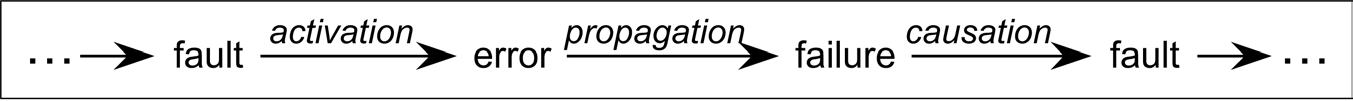
\includegraphics[width=0.65\textwidth]{figures/propagation.png}
\caption{The chain of dependability~\cite{art:Avizienis}}
\label{fig:propagation}
\end{figure}

Knowing what the dependability is and what are the threats, it is important to know what available \textbf{means} do developer have to create a dependable system. There are four solutions:
\begin{itemize}
    \item \textbf{Fault Prevention} aims mostly at the development phase of a system and relays on design rules, modularization and strongly-typed languages. It also records the detected faults and eliminates them through development process modification.
    \item \textbf{Fault Tolerance} stands for methods which imply the presence of faults and their inevitability. Hence the need for error detection and processing. The fault tolerance is elaborated in the~\autoref{sec:tolerance}.
    \item \textbf{Fault Removal} in the development phase has three stages: verification, diagnosis and correction. If the verification shows faults in the system, the two other steps need to be applied. The verification needs to be repeated afterwards. In the use phase the faults are removed through maintenance, which requires an external agent (a repairman, some test equipment or software).
    \item \textbf{Fault Forecasting} bases on evaluation process of the system behavior, especially the fault occurrence and activation. The evaluation can be either qualitative - classify and rank events that are dangerous to the system; or quantitative - count and give probabilistic measure of the extent in which the attributes of dependability are satisfied~\cite{art:Avizienis, art:Avizienis2}. 
\end{itemize}
While the fault prevention and the fault forecasting are more useful in analysis of the system dependability and aim to minimize the amount and severity of faults in the system, thus helping by the fault avoidance; the fault tolerance and fault removal both assume that the faults happen and provide methods to reduce their impact on the system, creating a group of fault acceptance methods, thus helping in handling the systems that are subject to faults. \autoref{fig:depgroup} represents the grouping of dependability means.

\begin{figure}[H]
\centering
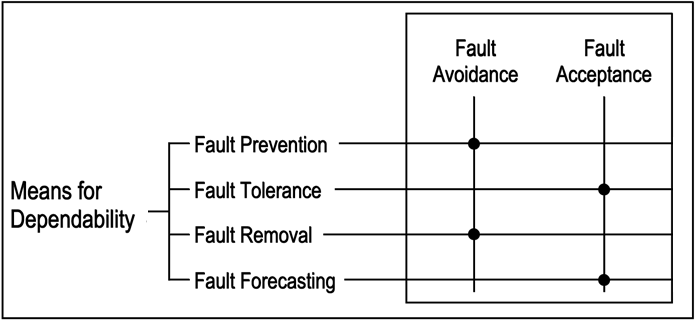
\includegraphics[width=0.65\textwidth]{figures/depgroup.png}
\caption{Grouping of the means for dependability~\cite{art:Avizienis}}
\label{fig:depgroup}
\end{figure}

%************************************************************************************************************************%
\section{Fault Pathology}
There are eight categories that help to understand what kinds of faults there are and how they may influence the system. They are called the elementary fault classes. Each fault falls into more classes. They may be understood as properties of a fault. The possible combinations are marked with a dot in the~\autoref{fig:fault}. The developer has to decide witch classes should be included in the dependability specification.

\begin{figure}[H]
\centering
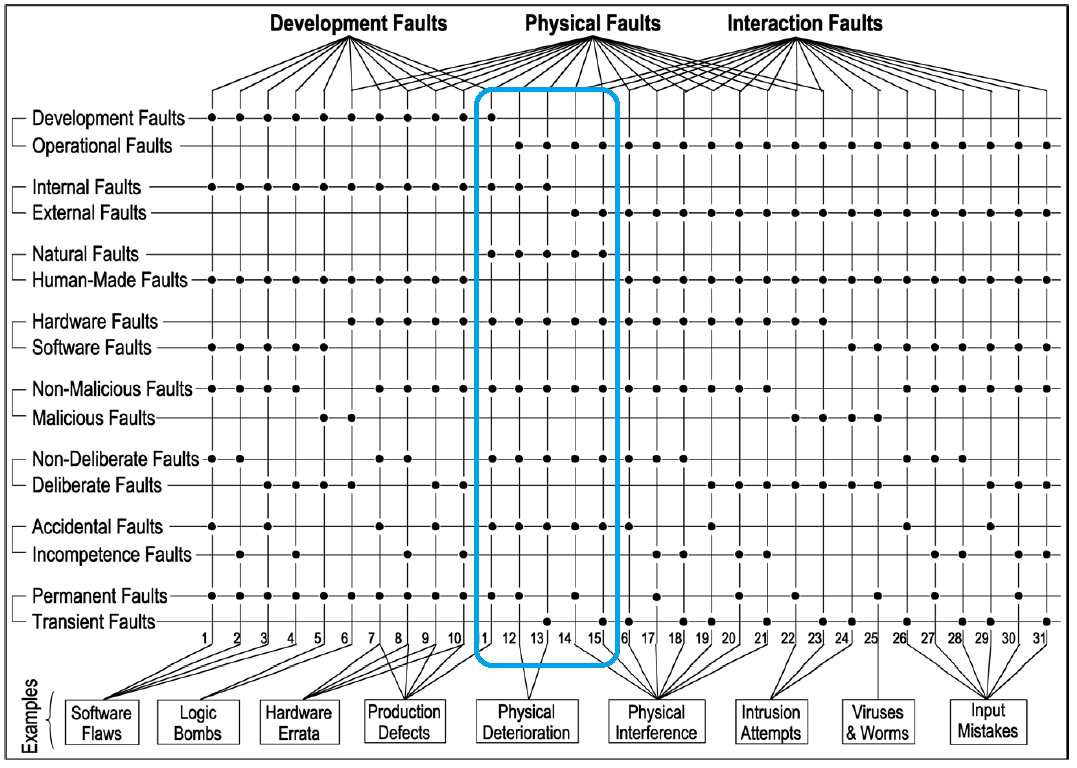
\includegraphics[width=\textwidth]{figures/fault_classes.png}
\caption{The elementary fault classes~\cite{art:Avizienis}}
\label{fig:fault}
\end{figure}

The classes divide into three main groups: the development faults, the physical faults and the interaction faults. The development faults occur during the development phase of the system. The last group describes faults that happen during the use phase and come from the use environment of the system, hence they are operational faults (excluding the internal faults). Physical faults are all faults that happen in hardware, they happen during the development and use phase invariably.
Very important perspective splits faults up into two, or actually three groups, based on the duration of the fault and its persistence:
\begin{itemize}
    \item The \textbf{transient faults} occur once and don't persist afterwards. The error caused by such a fault is called a soft error.
    \item The \textbf{permanent faults}, often called hard faults, occur at some point in time and last until the faulty component gets repaired. Faults occurrence may happen already in the development phase and results in erroneous data being produced by affected component during its use. 
    \item The \textbf{intermittent faults} occur repeatedly but not continuously in the same spot in the design. The errors caused by such faults tend to also be intermittent~\cite{book:Sorin}.
\end{itemize}
The knowledge about the faults persistence is therefore important, that it changes the strategy of fault tolerance. The permanent faults, to be removed, require some sort of repair procedure, while the transient faults require much less complicated treatment, like repetition of the operation.

Let's focus on faults that occur in hardware and are caused by natural phenomena. Those faults are marked with a box in the~\autoref{fig:fault}. There are three stages within this group:
\begin{itemize}
    \item Production defects - are all development faults which are permanent. These can be imperfections and variations in one of the production stages or dust particles causing shorts. They lead to functional and parametric errors and should be caught before the use phase. One of the possibilities is the burn-in test which consists in stressing the circuit with high temperature and voltage, leading to its premature aging. The early life failures are caught and affected circuit doesn't get to it's use phase.
    \item Physical Interference - are all external faults, both permanent, transient and intermittent caused by radioactive radiation and electromagnetic interference. These faults are randomly distributed throughout the whole life of a the system.
    \item Physical Deterioration - are the faults resulting from aging. They can be permanent, transient and intermittent. Electromigration (EM) and Stress Migration (SM) are just two of many possible aging effects by which an integrated circuit may be affected. The probability of such faults rises together with the systems age~\cite{art:Avizienis, art:Avizienis2}.
\end{itemize}
The~\autoref{fig:badewanne} shows the Fault rate/time relation. The first part of the diagram shows Early-Life-Failures, which result from the Production Defects. They should be captured during early life tests of the design. Next stage shows all faults happening due to Physical Interference. They are constantly threatening the system keeping the fault rate at the stable level. It may happen that systems environment is less or more "fault likely" but it would just shift the fault rate along the $y$ axis and not change its monotonicity. The last part shows a rising number of faults due to aging and deterioration processes happening to every hardware (and, according to some definitions also to software).

\begin{figure}[H]
\centering
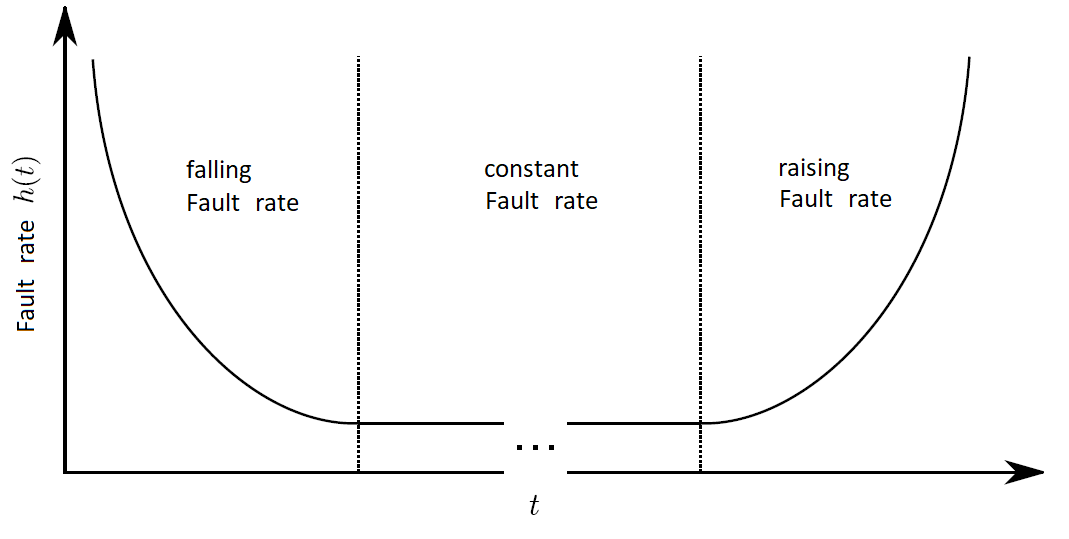
\includegraphics[width=0.65\textwidth]{figures/badewanne.png}
\caption{Fault rate throughout systems life cycle~\cite{art:Avizienis}}
\label{fig:badewanne}
\end{figure}


%************************************************************************************************************************%
\section{Fault Tolerance}\label{sec:tolerance}
The fault tolerance is one of the dependability means. The developer cannot only rely on fault avoidance methods because of the time needed for manual repair and frequency of those repairs. Sometimes the system is also inaccessible for maintenance. Additionally the more complex is the hardware, the more liable it is to natural faults. Thus while designing the hardware which is either very complex or doesn't allow long time to repair then the incorporation of fault tolerance is a must.\\
Fault tolerant systems can react differently in the presence of faults. Some provide the full performance, some offer just a reduced functional capability~\cite{art:Randell}. There are therefore different schemes of fault tolerance and they depend on the faults that are supposed to be tolerated. There are however two main parts that have to always exist: error detection and system recovery.\\
The error detection can either be concurrent to main functionality or happen during scheduled pauses, when normal functionality is suspended. After the error is detected the recovery routine has to deal with two problems. The first one is the error handling which can be performed via:
\begin{itemize}
    \item backward error recovery - executed on demand. The system is brought back to a saved state that is known to be error-free. This state has to be saved prior to error occurrence, thus its name is checkpointing.
    \item forward error recovery - also executed on demand. Finding a new state, which has not yet bee occupied by the system, which is error-free.
    \item error compensation - can be used either systematically (also in absence of faults) or on demand. The erroneous state contains enough redundancy to provide correct service despite the fault. The systematic usage is called the fault masking.
\end{itemize} 
The other problem is to remove the cause of an error, therefore the fault handling may be necessary. It consists of:
\begin{itemize}
    \item Diagnosis - identifies and stores the cause of an error and its location together with the time when the error happened.
    \item Isolation - excludes the faulty component from normal function either logically or physically 
    \item Reconfiguration - provides a spare component to take place of the faulty one or reassigns the tasks among non faulty components
    \item Reinitialization - logs the changes made in configuration and updates the records or system tables 
\end{itemize}
The coverage of fault tolerance is a measure of its successful detection of erroneous states associated with faults and its ability to repair or replace such states. Every method covers different faults and errors, therefore only a combination of them can lead to a maximum fault coverage.
Fault tolerance requires protective redundancy, being additional components and algorithms allowing the error detection and preventing errors from leading to failures. Unfortunately the fault tolerance is a recursive procedure, witch means that every redundancy, when implemented, becomes part of the system, and therefore can be affected by all previously described faults.
There are four main arts of redundancy: time redundancy, hardware redundancy, software redundancy and information redundancy. The software redundancy will not be discussed.
%************************************************************************************************************************%
\subsection{Hardware Redundancy} \label{ssec:HWred}
The main overhead lies in hardware. The components are either passive or active. 

The passive redundancy aims for immediate masking of a failure. As long as the number of faults doesn't exceed the specified maximum, the system provides correct functionality without showing any kinds of disturbance. It's achieved through a parallel execution of operations on more concurrent components in hope that faults appear independently in each one of them. An example of such art of redundancy is the N-Modular Redundancy system, which has N modules running in parallel and majority voter that propagates the result that occurred in the majority of the modules. A variation of such system would incorporate more voters running in parallel to eliminate the single-point-of-failure, which is the voter in an NMR system. Passive redundancy is an example of error compensation without any sort of fault handling but with systematic error detection, which happens inside of the voter. The permanent faults are masked as long as their accumulation with transient faults doesn't exceed the coverage of the system.

The active redundancy is a way to solve the permanent fault problem which occurs in passive redundancy. After error detection, the erroneous component is localized and replaced by a fault-free spare component. The start procedure of such a component can take some time, that could be avoided if the component had worked in parallel to the rest of the system by the time of error occurrence. Such strategy is called a Hot-Standby (in opposite to Cold-Standby) but it leads to component deterioration, without it being actually used for the main functionality. The active redundancy is an example of rollforward approach, since the configuration after repair is a state that has not been used before the error occurrence. The error detection can be either systematical or happen in intervals, depending on the requirements.

There is a possibility to combine both approaches to a hybrid one. Having a systematical error compensation with an active spare modules. Once a permanent fault is detected a reconfiguration takes place, either on-line or during a break.


%************************************************************************************************************************%
\subsection{Time Redundancy}
This type of redundancy has a very powerful advantage, namely it doesn't require so much additional hardware. The time redundancy is mostly implemented in software, that executes operations more times in a row achieving the same result as the hardware redundancy without its cost. With 2 repetitions the errors can be detected and three repetitions allow error correction. The repetitions can be achieved through a checkpoint system. The repetitions may also happen concurrently on different threads leading to use different processor resources for the same task and creating a quasi NMR system. For transmission errors the \textbf{Error Correction Through Retransmission} is possible. It's based on an assumption, that after the detection of an error, there is enough time to retransmit the information. The redundancy results in the additional control bits for error detection (information redundancy) and in the additional time for retransmission.

%************************************************************************************************************************%
\subsection{Information Redundancy}\label{ssec:Infred}
The information flow through a system can be corrupted by many different faults. Other proposed methods try to not let to the information integrity violation. But maybe even if the information got changed, then there is a possibility to detect this change and reconstruct the original information. The information redundancy tries to achieve exactly this goal by adding some special parity bits to detect or even correct the errors. Special codes make it possible to achieve this goal.

\textbf{Backward Error Correction} (BEC), more commonly called Automatic Repeat Request (ARQ) allows the detection of errors in the information and requires the retransmission. The codes used in this approach are called Error Detecting Codes (EDC)

\textbf{Forward Error Correction} (FEC) enables localization of the error position within the information and as a result, reconstruction of the original information, without the need of retransmission. The only redundancy are the control bits and the encoder/decoder pair (Hardware or Software). The codes used in this approach are called Error Correcting Codes (ECC)~\cite{book:SchonfeldKlimant}.

%************************************************************************************************************************%
\section{Channel Coding} \label{sec:cod}
In the year 1948 Shannon published a landmarking paper "Mathematical Theory of Communication" where he showed that, with a certain information encoding, the errors induced by a noisy channel can be reduced to any suitable level~\cite{art:Shannon}. With this article he started the era of coding theory and a race to create better and better codes with simple decoding algorithms~\cite{book:Lint}. He laid the mathematical foundation of reliable communication, without indication how to construct the codes and build optimal encoders and decoders.\\

Channel Coding is, generally speaking, a process of adding useful redundancy to the source information in order to recreate it's contents after it arrives at the sink. ECC are used to supervise memory interfaces, hardware operations and wireless communication. Each use case requires different properties of the code. The memory transactions and hardware operations focus on single and double bit errors, while wireless communication needs to handle multiple bit errors. Additionally the implementation of encoding and decoding can either take place in hardware or in software, which implies different complexity and power consumption, but most importantly the execution time and therefore the latency. With the wireless communication replacing the wired connections, the demand on short and efficient coding algorithms moves the processing of the information into hardware. 

\subsection{Error Detection}
To conduct any error correction, the error detection has to take place first. Let's assume that the information leaving the source encoder is a binary sequence that can be divided into blocks of length $k$. Each block is denoted as 
$$u=(u_1,u_2,...,u_k)$$ 
and is called a \textit{message} with \textit{k user bits} . Since the information is binary, there are $2^k$ different messages possible. The channel encoder transforms each $message$ into a binary \textit{code word}. In the systematic code, where the information is added at the end of the $message$, the \textit{code word} looks as follows:
$$v=(v_1,v_2,...,v_{n+k}) = (u_1,u_2,...,u_k, c_0,c_1,...,c_{n})$$ 
with length $n+k$. There are \textit{n check bits} appended to the \textit{user bits}. There are only $2^k$ valid \textit{code words}, since every \textit{code word} corresponds exactly to one $message$. The set of all valid \textit{code words} is called a code space. It leaves $2^n$ \textit{words} that are not used in transmission and are invalid. The ratio $R=k/(n+k)$ is called the \textit{code rate} and can be understood as the number of the information bits entering the encoder per transmitted symbol. During the transmission, an \textit{error vector e} overlays the \textit{code word u} producing a \textit{received sequence v'} 
$$e=(e_1,e_2,...,e_{n+k})$$ 
$$v'=(v'_1,v'_2,...,v'_n)= (e_1 \oplus v_1, e_2 \oplus v_2,...,e_{n+k} \oplus v_{n+k})$$

If the \textit{received sequence} is not a valid \textit{code word}, then the error gets detected. The worst case scenario is when the \textit{error vector} transforms a \textit{code word} into a valid \textit{received sequence} but different then the \textit{code word} sent, $v'\neq v$. Then the \textit{received sequence} gets accepted and decoded into a wrong $message$. To avoid such situations, the \textit{code words} should lay possibly away from each other. It means that they should differ in as many places as possible. The \textit{hamming distance d} (between two \textit{code words}) is the number of positions, in which both words differ. The number of errors $f_d$, that a code can detect, depends on the minimum hamming distance $d_{min}$ in the code space, which has to satisfy following inequality $d_{min} \geq f_d + 1$.
\subsection{Error Correction}
If the \textit{code word} overlaid with \textit{error vector} results in the \textit{received sequence} outside of the code space, then the error gets detected. The~\autoref{fig:hamming_dist} shows the hamming distance cube for a 3 bit binary word. Each vertex symbolizes a possible \textit{received sequence}, where only words $\{000\}$ and $\{111\}$ are valid \textit{code words}. The distance between the words is equal to the number of edges between them. The hamming distance between the \textit{code words}, being the \textit{minimum hamming distance} is in this case $d_{min}=3$.

\begin{figure}[H]
\centering

\includegraphics[width=0.3\textwidth]{figures/Hamming_distance.png}
\caption{Hamming distance cube for 3-bit binary numbers~\cite{web:hamming_dist}}
\label{fig:hamming_dist}
\end{figure}

Assuming that the number of errors is $f_c = 1$, then upon reception of erroneous data, the distance between the \textit{received sequence} and valid \textit{code word} will also be $d = 1$. The \textit{received sequences} form therefore two disjoint sets $r_{000}=\{001,010,100\}$ and $r_{111}=\{110,101,011\}$, where $r_{000}$ represents all possible received messages, corrupted by single bit error, upon sending the $\{000\}$ message and the $r_{111}$ - upon sending the $\{111\}$ message. The reception of any word from each set unambiguously refers to only one valid \textit{code word} (assuming the minimum distance decoding scheme), that could have been sent, hence the error correction is possible. To correct $f_c$ errors the code needs to have $d_{min} >= 2f_c+1$. If the $d_{min}$ is even, then there will always be some words in the \textit{received sequence set} that have equal distance to more than one \textit{code word}, making the correction impossible. If the $d_{min} = 2f_c+1$, the code is called perfect. A perfect code is an optimal code, where every \textit{received sequence} can be unambiguously subordinated to a valid \textit{code word}. The distances between all code words are equal and maximal. The code has to satisfy the following equality $k=ld\sum_{i=0}^{f_c} \binom{n}{i}$ to be called a perfect code. Perfect codes use their redundancy fully, guaranteeing maximal protection by minimal overhead.

\subsection{Types of Codes}
For the last 70 years, scientists have developed many codes, that suit different purposes. Let's focus on binary codes, that are constructed from an alphabet \{0,1\}. In hardware dependability, there are two main fields of application and therefore two groups of codes:
\begin{itemize}
\item The Hamming code~\cite{art:Hamming}, with the ability of detection and correction of single bit errors and its extended version for double error detection and single error correction (DED-SEC) and the Hsiao code~\cite{art:Hsiao}, which is also a DED-SEC code. They are both widely used in hardware supervision, like memory interfaces. They are linear block codes, which means that the source information is split into blocks and coded with utilization of linear boolean functions only (XOR operations), therefore all codewords are linear combinations of each other. Hence they are commonly referred as vectors, from linear algebra. The decoding can happen within one clock cycle, which is necessary in protecting hardware interfaces.  
\item The BCH code, as a multiple bit error correcting code, with significantly longer decoding time then DED-SEC codes. It uses a hard decision decoding scheme based on "hard coded" algebraic functions, in this case a polynomial division with use of LFSR. It is a linear cyclic code, where all codewords are not only linear combinations of each other, but also every code word is just a shifted version of another one. This code is used in wireless communication because of it ability of multiple bit error correction.\\
The Low Density Parity Codes (LDPC)~\cite{art:LDPC} and Turbo codes~\cite{art:turbo} are the examples of soft decision methods, where the best candidates for correct code words are identified and then selected by majority voters. They take longer decoding time then BCH codes, but as few other codes, they come very close to the Shannon's limit, allowing highest information throughput within noisy channels. They also contain many memory cells, exposing them to transient faults.\\
\end{itemize}

\subsection{Construction of a SEC-DED Hsiao Code}\label{sec:Hsiao}
While the theory behind ECC is well known and was introduced already almost 70 years ago, the creation of optimal codes is still a subject to the intensive research. The ease of implementation and short execution times combined with the high protection against errors are the key factors in creating codes. Since the code detection and correction capabilities are strongly dependent on the minimal hamming distance, the creation of codes focuses on keeping the maximal distance by minimal code word length. In linear codes the creation of check bits results from linear operations on the user bits. The check bits are in fact group parity bits that may be implemented in hardware as simple XOR operations. The specific user bits that take part in calculation of every check bit can be represented using the generator matrix $G$. The generator matrix for Hsiao Code is shown below:
\begin{equation*}
\underbrace{
\vphantom{\bordermatrix{&&&&&&&&\cr &1&0&0&0&1&1&1&0\cr&0&1&0&0&0&1&1&1\cr&0&0&1&0&1&0&1&1\cr&0&0&0&1&1&1&0&1\cr}
}(u_0,u_1,u_2,u_3)}_{u}
\cdot 
\underbrace{\bordermatrix{
&v_0&v_1&v_2&v_3&v_4&v_5&v_6&v_7\cr 
&1&1&1&0&1&0&0&0\cr
&0&1&1&1&0&1&0&0\cr
&1&0&1&1&0&0&1&0\cr
&1&1&0&1&0&0&0&1\cr
}}_{G_{4\times 8}} = 
\underbrace{
\vphantom{\bordermatrix{&&&&&&&&\cr &1&0&0&0&1&1&1&0\cr&0&1&0&0&0&1&1&1\cr&0&0&1&0&1&0&1&1\cr&0&0&0&1&1&1&0&1\cr}
}(c_0,c_1,c_2,c_3,u_0,u_1,u_2,u_3)}_{v'}
\end{equation*}
The number of columns in the generator matrix specifies the length of the code word and the rows correspond to the number of user bits. The multiplication of the user bit vector with the generator matrix results in following check bits: 

\begin{align}
\begin{aligned}
c_0 &= u_0 \oplus u_2 \oplus u_3  \\
c_1 &= u_0 \oplus u_1 \oplus u_3  \\
c_2 &= u_0 \oplus u_1 \oplus u_2  \\
c_3 &= u_1 \oplus u_2 \oplus u_3 
\end{aligned}
\end{align}

Every check bit depends on three user bits, visible as three ones in the corresponding columns of the G matrix. The matrix contains an identity matrix, responsible for the presence of the user bits in the code word.

The linear codes are most commonly represented by their parity-check matrices $H$, from which all code properties can be derived. While the generator matrix describes the encoding operation, the parity check matrix is used to decode the received sequence $v'$ into an error-free message. The $H$ matrix of a DED-SEC Hsiao Dode looks as follows:
\begin{equation*}
\underbrace{
\vphantom{\bordermatrix{&&&&&&&&\cr &1&0&0&0&1&1&1&0\cr&0&1&0&0&0&1&1&1\cr&0&0&1&0&1&0&1&1\cr&0&0&0&1&1&1&0&1\cr}
}(c_0',c_1',c_2',c_3',u_0',u_1',u_2',u_3')^T}_{v}
\cdot \underbrace{\bordermatrix{
&&&&&&&&\cr 
 s_1 &1& 0 & 0 & 0 &1&0&1&1 \cr 
 s_2 &0& 1 & 0 & 0 &1&1&0&1 \cr 
 s_3 &0& 0 & 1 & 0 &1&1&1&0\cr 
 s_4 &0& 0 & 0 & 1 &0&1&1&1
}}_{H_{4\times 8}} = 
\underbrace{
\vphantom{\bordermatrix{&&&&&&&&\cr &1&0&0&0&1&1&1&0\cr&0&1&0&0&0&1&1&1\cr&0&0&1&0&1&0&1&1\cr&0&0&0&1&1&1&0&1\cr}
}(s_1,s_2,s_3,s_4)^T}_{\text{syndromes}}
\end{equation*}

The number of columns is equal to the length of the code word, and the number of rows denotes the number of check bits. The number of 1-positions in each column is odd and the hamming distance between any two rows is kept equal 1. There is also a minimal number of 1-positions in the whole matrix. There is no column with all zeros and every column is distinct. If the requirements are met, the code has a minimal distance of $d_{min} = 4$. The result of multiplying the received sequence vector with the parity check matrix is called the syndrome. Syndromes get calculated in the following way:

\begin{align}
\begin{aligned}
s_1 &= u_0' \oplus u_2' \oplus u_3' \quad\oplus c_0' \\
s_2 &= u_0' \oplus u_1' \oplus u_3' \quad\oplus c_1' \\
s_3 &= u_0' \oplus u_1' \oplus u_2' \quad\oplus c_2' \\
s_4 &= u_1'\oplus u_2' \oplus u_3' \quad\oplus c_3' \\
\end{aligned}
\end{align}

The order of operations has been deliberately changed to show that the computation of syndromes consists of two stages. Firstly the received user bits are processed by the embedded encoder in the decoder system and the check bits from received user bits are derived. This are the operations on user bits. The calculated check bits are compared with the received check bits and the error syndrome is created. Any non zero value of the syndrome indicates some sort of error in the received vector. Let's analyze the steps to understand how syndromes may be used for error detection and correction. 

In case that an error appeared in one of the user bits, there will be exactly 3 non zero syndromes. The only syndrome remaining zero, will be the one that does not involve the faulty bit in its computation. In case of an error in $u_1'$ it will be $s_1$, for $u_2'$ - $s_2$, for $u_3'$ - $s_3$ and for $u_0'$ - $s_4$. The syndrome therefore is exactly equal to the column in the $H$ matrix that corresponds to the faulty user bit. To repair the error, the appropriate user bit needs to be simply flipped. The code is capable of locating and repairing one bit errors.

In case of a single error in one of the received check bits, exactly one syndrome, associated with this check bit, will be non-zero. $s_1$ for $u_0'$, $s_2$ for $u_1$, etc. This situation doesn't require any correction, since all user bits are error-free. 

In case of a double error in user bits or one user bit and one check bit, the result will be two syndromes equal 1. There is no way to tell which bits were flipped, since more combinations result in the same syndrome configuration. Hence double error detection, without correction.

For three errors the number of non-zero syndromes will be either 1 or 3, exactly as in the case of single bit errors. This situtation leads to mis-correction and cannot be detected in this form of code. Assuming that three user bits were faulty, exactly one syndrome will be non zero. The decoder will assume, that it was more probable, that the parity bit was flipped then all user bits creating this bit and it will correct the parity bit. The result will be 4 errors. Also in all other combination of triple bit errors, the decoder will produce one additional error on top.

The Hsiao Code is a SEC-DED code, where an odd number of errors produces an odd number of flipped syndromes and an even number of errors - an even number of non-zero syndromes. Every multiple-bit error, with hamming weight greater then 2 can trigger a false repair or in case of even number of errors, it can get accepted as fault free. The number of ones in the parity check matrix corresponds to the number of XOR gates required to implement the code functionality, the weight of a single row in the H matrix specifies the number of levels (subsequent gates) that the signal need to pass from input register to output register of the decoder. The Hsiao Code is known from its minimal number of ones in the parity check matrix and therefore minimal hardware overhead for en- and decoding. The lower the number of gates, the lower not only the power consumption and execution time, but also the error rate, since the probability of errors rises together with the hardware complexity.

\section {ParSec Communication System}
Various signals transmitted in industrial environment have different requirements in terms of dependability. Let's consider a simple CCTV video transmission system. Each frame, even in low resolution solutions, consists of several hundred thousands pixels. The frame rate lies somewhere between 30 and 5 frames per second, depending on the requirements. Even multiple bit error in the compressed video information bitstream leads just to the corruption of some frames. Depending on the error rate and frame rate, such disturbance may not influence the correct service at all, just lowering the video quality. The system, despite some errors, still fulfills it's function.

On the other hand the information flow between the control system and the nodes, placed on the robotic arms on the assembly line, consists in constant transmission of the coordinates of the destination and position of the arm. An error in such information can lead to the damage of manipulated objects or another catastrophic system failure.

Moreover, the quality of the signal propagation in such a rapidly changing environment is not constant. The error rate can significantly rise for a short time, but be relatively low otherwise. Spending time, power and resources on complex encoding and decoding may not be justified for the majority of the systems life time. The ability to adapt to the quality of the transmission would be just another advantage of well designed communication system.

In conclusion, the requirements of the industrial wireless system are diversified and need a configurable solution, that could offer a constantly high level of dependability while adapting to its environment and the use case. The high level of dependability means the coverage of the hardware faults in the first place, since they can even prevent the establishment and synchronization of the connection.

The goal of the ParSec project is to create a dependable, flexible and secure wireless communication system which meets all industrial automation requirements. It has to work with latencies below 1 ms and with very high noise level, serving many distributed clients at once. Moreover it has to deal with fading effects and potentially many reflections or even obstacles coming in the way of transmission and breaking it.

The ParSec communication system (shown in~\autoref{fig:ParSec}) consists of the MAC Layer processing, taking place within a standard processor, implemented mostly as software routines, followed by the a FEC unit and by a frame formatter. The last part is the baseband processor, which consists of mixed and analog signal processing and Radio Frequency unit. 

\begin{figure}[h]
\centering
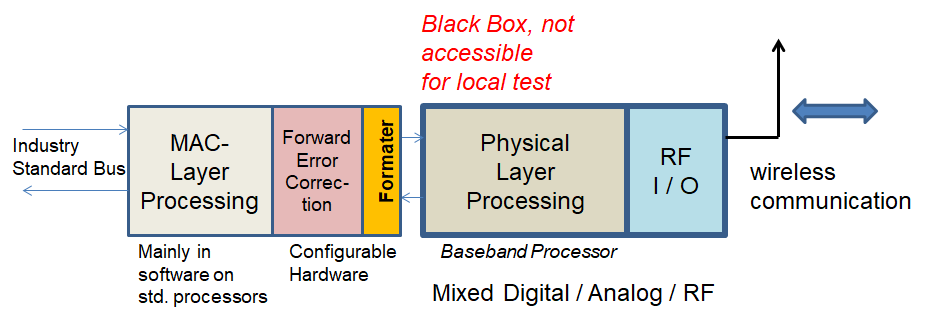
\includegraphics[width=0.65\textwidth]{figures/ParSec.png}
\caption{Block Diagram of the ParSec communiaction system}
\label{fig:ParSec}
\end{figure}

Both, the communication errors and soft errors due to transient faults in hardware, laying between FEC encoder and decoder, can be indifferently corrected thanks to ECC, as long as their number doesn't exceed the ECC correction capabilities. 

There are many techniques to improve the signal quality and make it resistant to fading effects due to multi-path signal propagation, poor signal-to-noise ratio or interferences, lowering the error rate. The known and used techniques involve Orthogonal Frequency Domain Multiplexing (OFDM) \cite{book:OFDM,art:OFDM}, Spread-Spectrum Communication \cite{art:spread-spectrum96,art:spread-spectrum97} or Ultra Wide-Band Frequency Communication \cite{book:ultra-wide08,book:ultra-wide04}. The OFDM technique would be suitable, but it ruquires many very fast AD converters~\cite{art:PSSS04}. The solution chosen for ParSec project is the Parallel Sequence Spread Spectrum (PSSS) technology~\cite{art:PSSS15,art:PSSS04,patent}. It provides comparable transmission quality as OFDM, without the cost of expensive AD converters.

The theory behind the creation of Error Correction Codes (ECC) has been presented in \autoref{sec:cod}. The detection and correction of single bit errors can be achieved using a simple Hamming code \cite{art:Hamming}. With Hsaio Code or extended Hamming Code the single error correction and double error detection is possible \cite{book:Fujiwara,art:Hsiao}. Unfortunately in such a noisy and harsh environment as industrial production site, there may be faults causing more than one or two bit flips in the data bit stream. For such purposes the multiple-bit correcting codes like Reed-Solomon code \cite{art:Reed-Solomon} or BCH Code \cite{art:BCH} are suggested. They typically require much more effort in  encoding and especially in decoding the information. They tend to be slower. There are also other methods to deal with correction of two-bit errors like \cite{art:Hosp, art:Varghese}. All these proposals lack a simple one-fits-all solution, that could be used and configured to the needs of the target system and it's environment.

The FEC in ParSec project is realized thanks to the Programmable Encoder Architecture (PENCA) designed by P. Pfeifer, firstly introduced in \cite{art:Pfeifer}, showed in~\autoref{fig:PENCA}. It is an answer to the strict requirements of the dependable communication systems. The core of the solution consists in the "honeycomb" structure of units. The units can be replaced by neighboring units in case of errors detected in one of them. The internal test can be performed automatically or on demand. After testing, the unit can be marked as faulty, once the test fails, and its functionality logically remapped into another unit. Both the input and output units are implemented in two copies, since they are single points of failure and in case of permanent fault detected wouldn't be able to get repaired without a spare. The control of the system is done through the microcode (secured with parity bits). But above all, the architecture can be configured to serve as different channel encoders, starting with the implementation of the single error correcting codes and ending with the multiple-bit error correcting codes or even cross-parity codes. It is done via generation of polynomials by each unit and sometimes even borrowing resources from neighboring units for more extended polynomial generations. Each unit being able to perform BCH generator polynomial length task up to 42 coefficients (34 BCH codes) or 65 coefficients (50 BCH codes) with borrowed resources.

 \begin{figure}[h]
 \centering
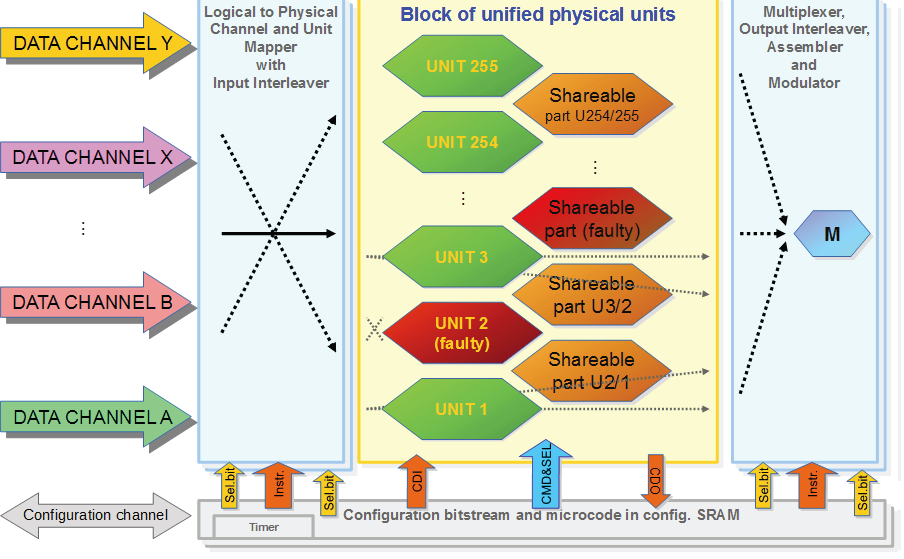
\includegraphics[width=0.65\textwidth]{figures/PENCA.png}
\caption{Basic scheme of the new dependable PENCA architecture~\cite{art:Pfeifer}}
\label{fig:PENCA}
\end{figure}

\section{FEC limitations}\label{sub:limits}
ECC can only be utilized in an environment, where the input information is equal to the output information. It is therefore a perfect solution for memory operations or communication, but it is hard to protect logical or arithmetic operations against transient faults or to detect permanent faults with use of ECC only. The special predictors can be used to evaluate the expected output of an operation, but they may prove to be almost as expensive, in terms of resources, and complicated as the protected units. In wireless communication, the transient faults and parameter shifts in digital and analog hardware modules laying between encoder and decoder are masked by the ECC used for transmission. The error detection within each module requires almost a duplication in hardware because their outputs are not comparable with their inputs.

Every permanent fault will lower the error detecting and correcting capabilities of the FEC system. Moreover in environments with higher error rates, like industrial communication systems, there is a need for multiple error correcting codes. In case of a multiple-bit errors in systems with not sufficient detecting capabilities, the errors may get accepted by the receiver without being aware of errors or it may conduct a miscorrection. On the other hand, the main drawback of multiple error correcting and detecting codes is their long and costly encoding and decoding. In the past the FEC operations could have been implemented in software, but after wireless communication entered real-time systems, with short latencies and no error acceptance, due to safety critical operations, the implementation of such operations inevitability moved to hardware. The operation executions in hardware are always faster and more energy efficient, but the algorithms become subjects to hardware faults. Although the processors executing all software routines have always been afflicted by hardware faults effects and should have been protected by any sort of redundancy, like time for re-execution to simulate an NMR system or parallel execution on more threads to create a real NMR system, the specialized hardware falls out of the coverage of processors fault tolerance and requires individual treatment. The next chapter describes methods for implementing different redundancies for diagnostic test purposes and for conducting repair operations in presence of permanent faults.

